\chapter{Docker와 웹앱}
좋습니다! 이제 docker run을 살펴보고 Docker 컨테이너를 사용해 보았으며 몇 가지 용어에도 익숙해졌습니다. 이 모든 지식을 바탕으로 이제 실제 작업을 시작할 준비가 되었습니다. 즉, Docker를 사용하여 웹 응용 프로그램을 배포하는 것입니다!

\section{정적 사이트}
작은 단계부터 시작해 봅시다. 첫 번째로 살펴볼 것은 매우 간단한 정적 웹사이트를 실행하는 방법입니다. Docker Hub에서 Docker 이미지를 가져와 컨테이너를 실행하고 웹 서버를 실행하는 것이 얼마나 쉬운지 확인할 것입니다.

시작해 봅시다. 우리가 사용할 이미지는 이번 데모를 위해 이미 생성된 단일 페이지 웹사이트이며 레지스트리에 호스팅되었습니다. 이미지를 한 번에 다운로드하고 실행할 수 있습니다. --rm 플래그는 컨테이너가 종료될 때 자동으로 제거되며, -it 플래그는 대화형 터미널을 지정하여 Ctrl+C로 컨테이너를 쉽게 종료할 수 있습니다.

\begin{figure*}[h]
  \centering
  \subfloat[]{%
    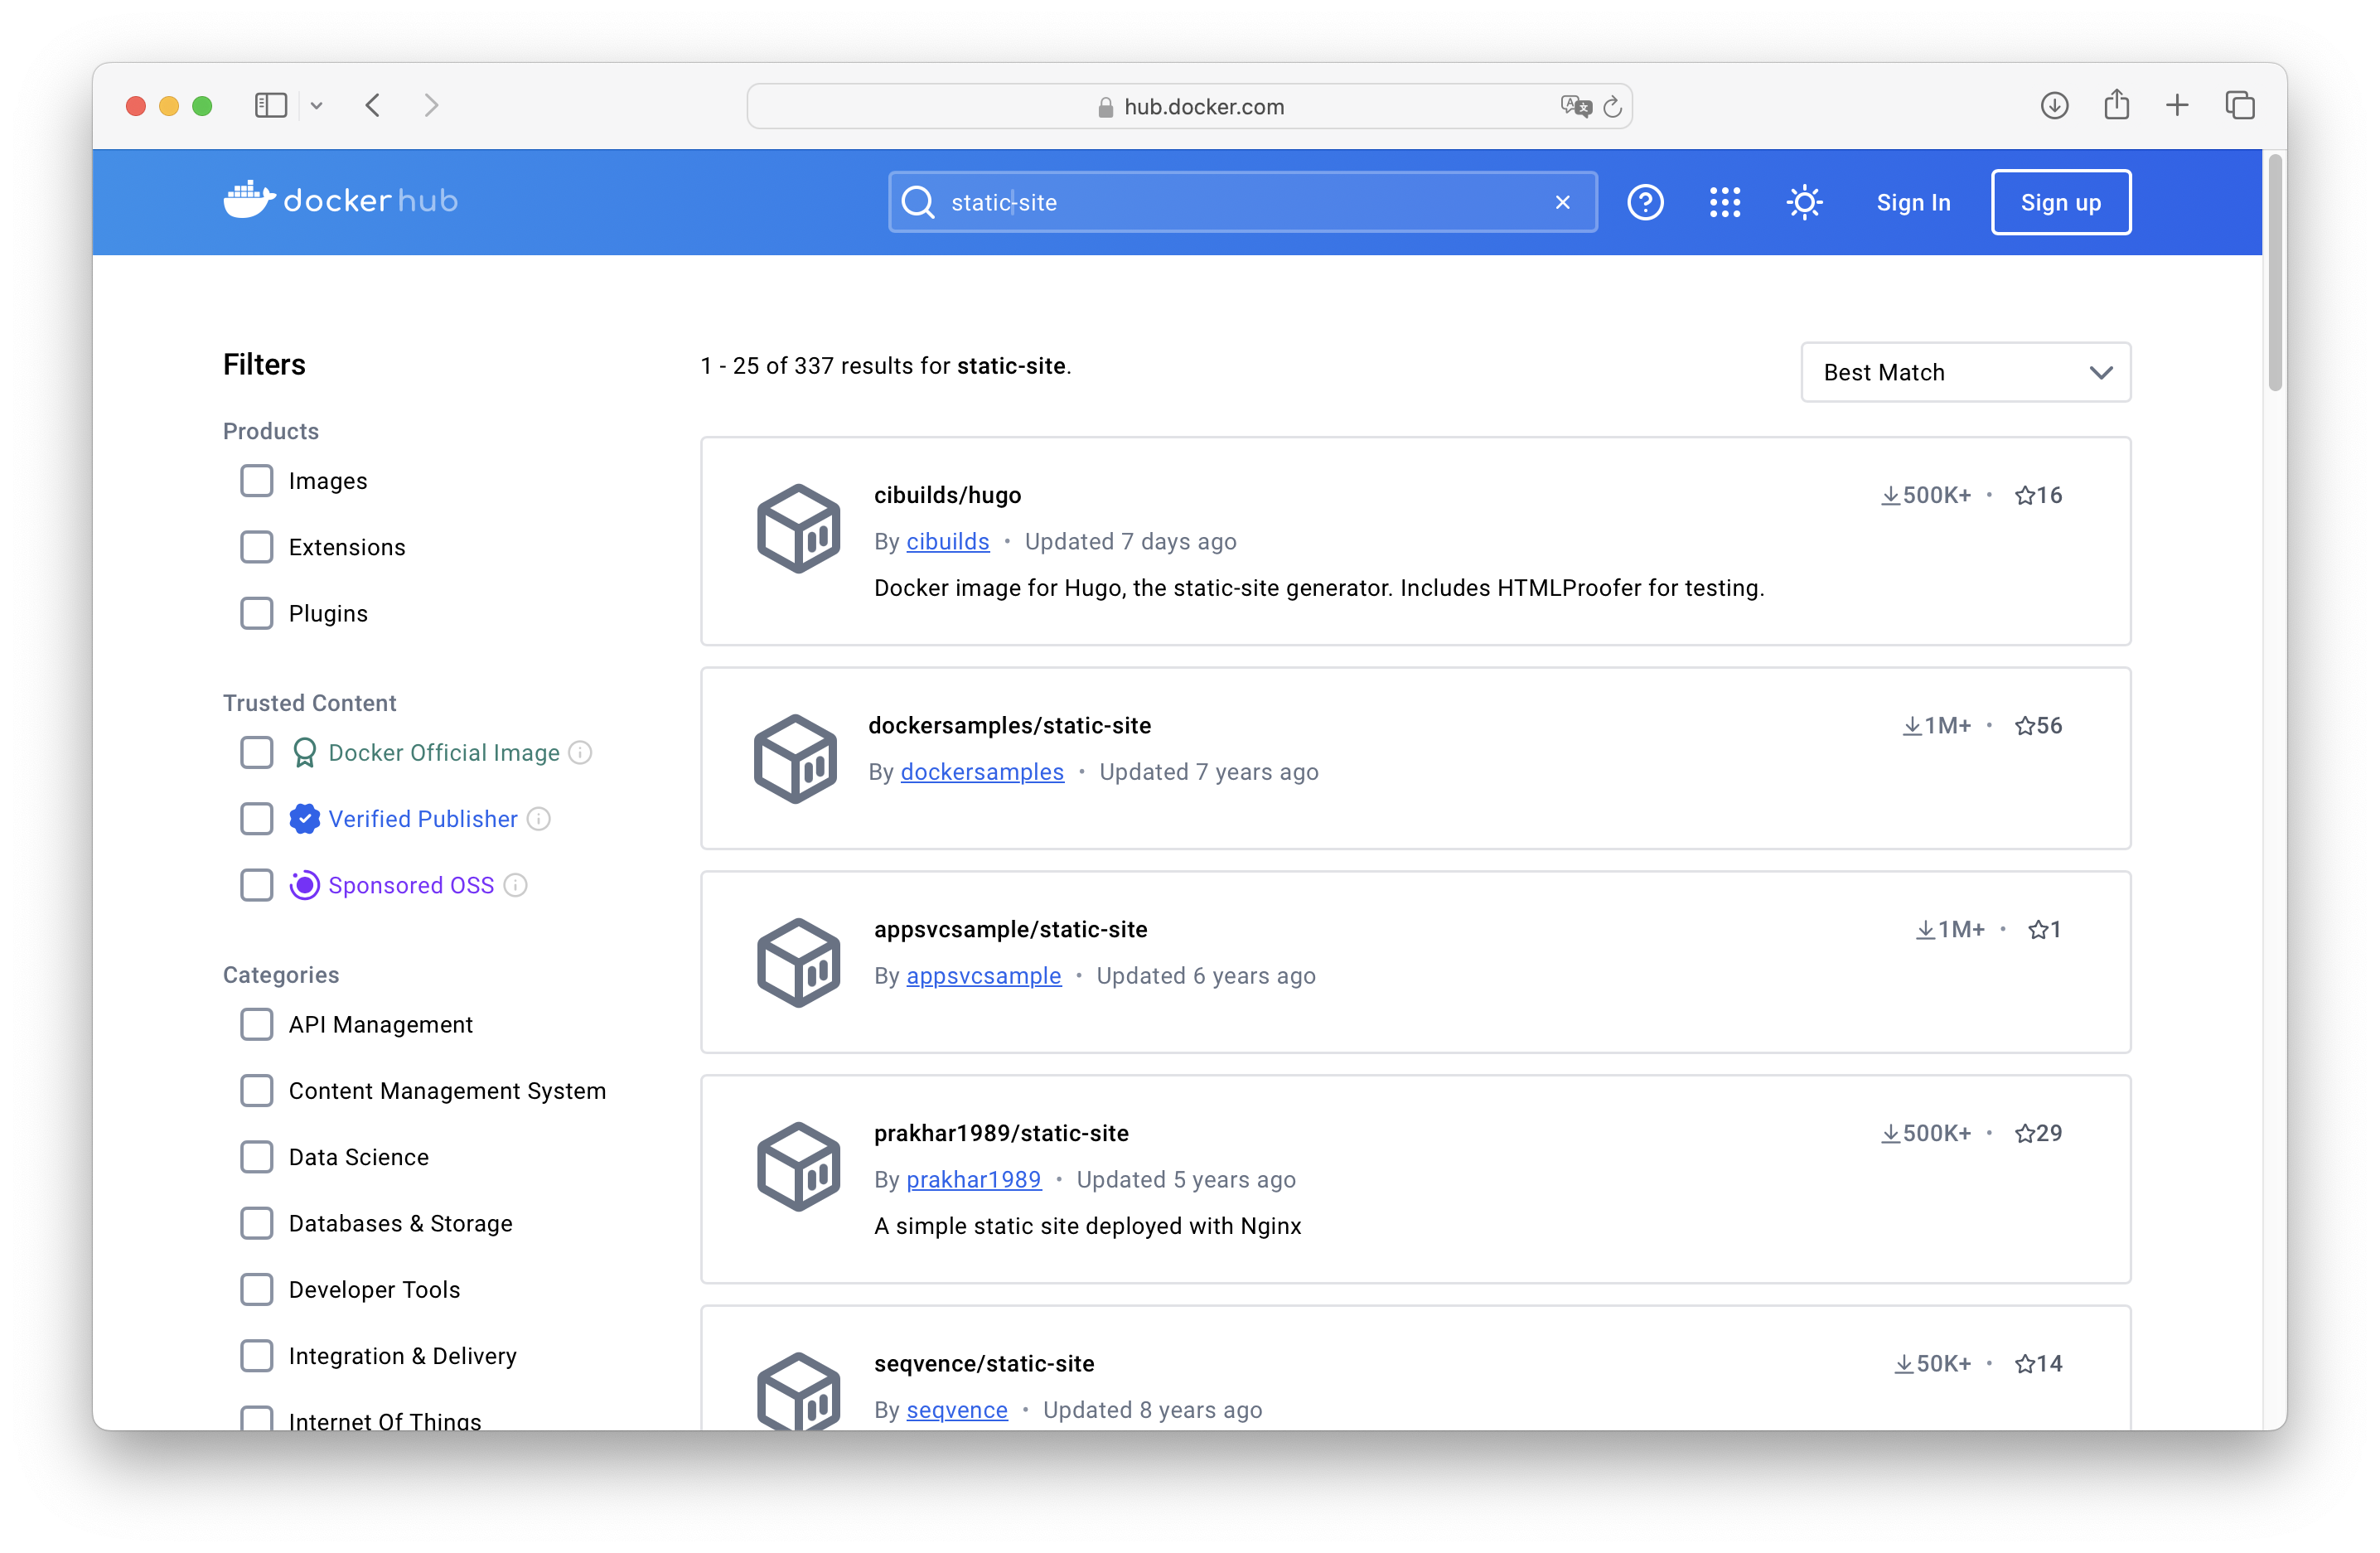
\includegraphics[width=.45\textwidth]{images/chapter4Images/ch4-1.png}
    \label{fig:nrGroup}
  }
  \hfill
  \subfloat[]{%
    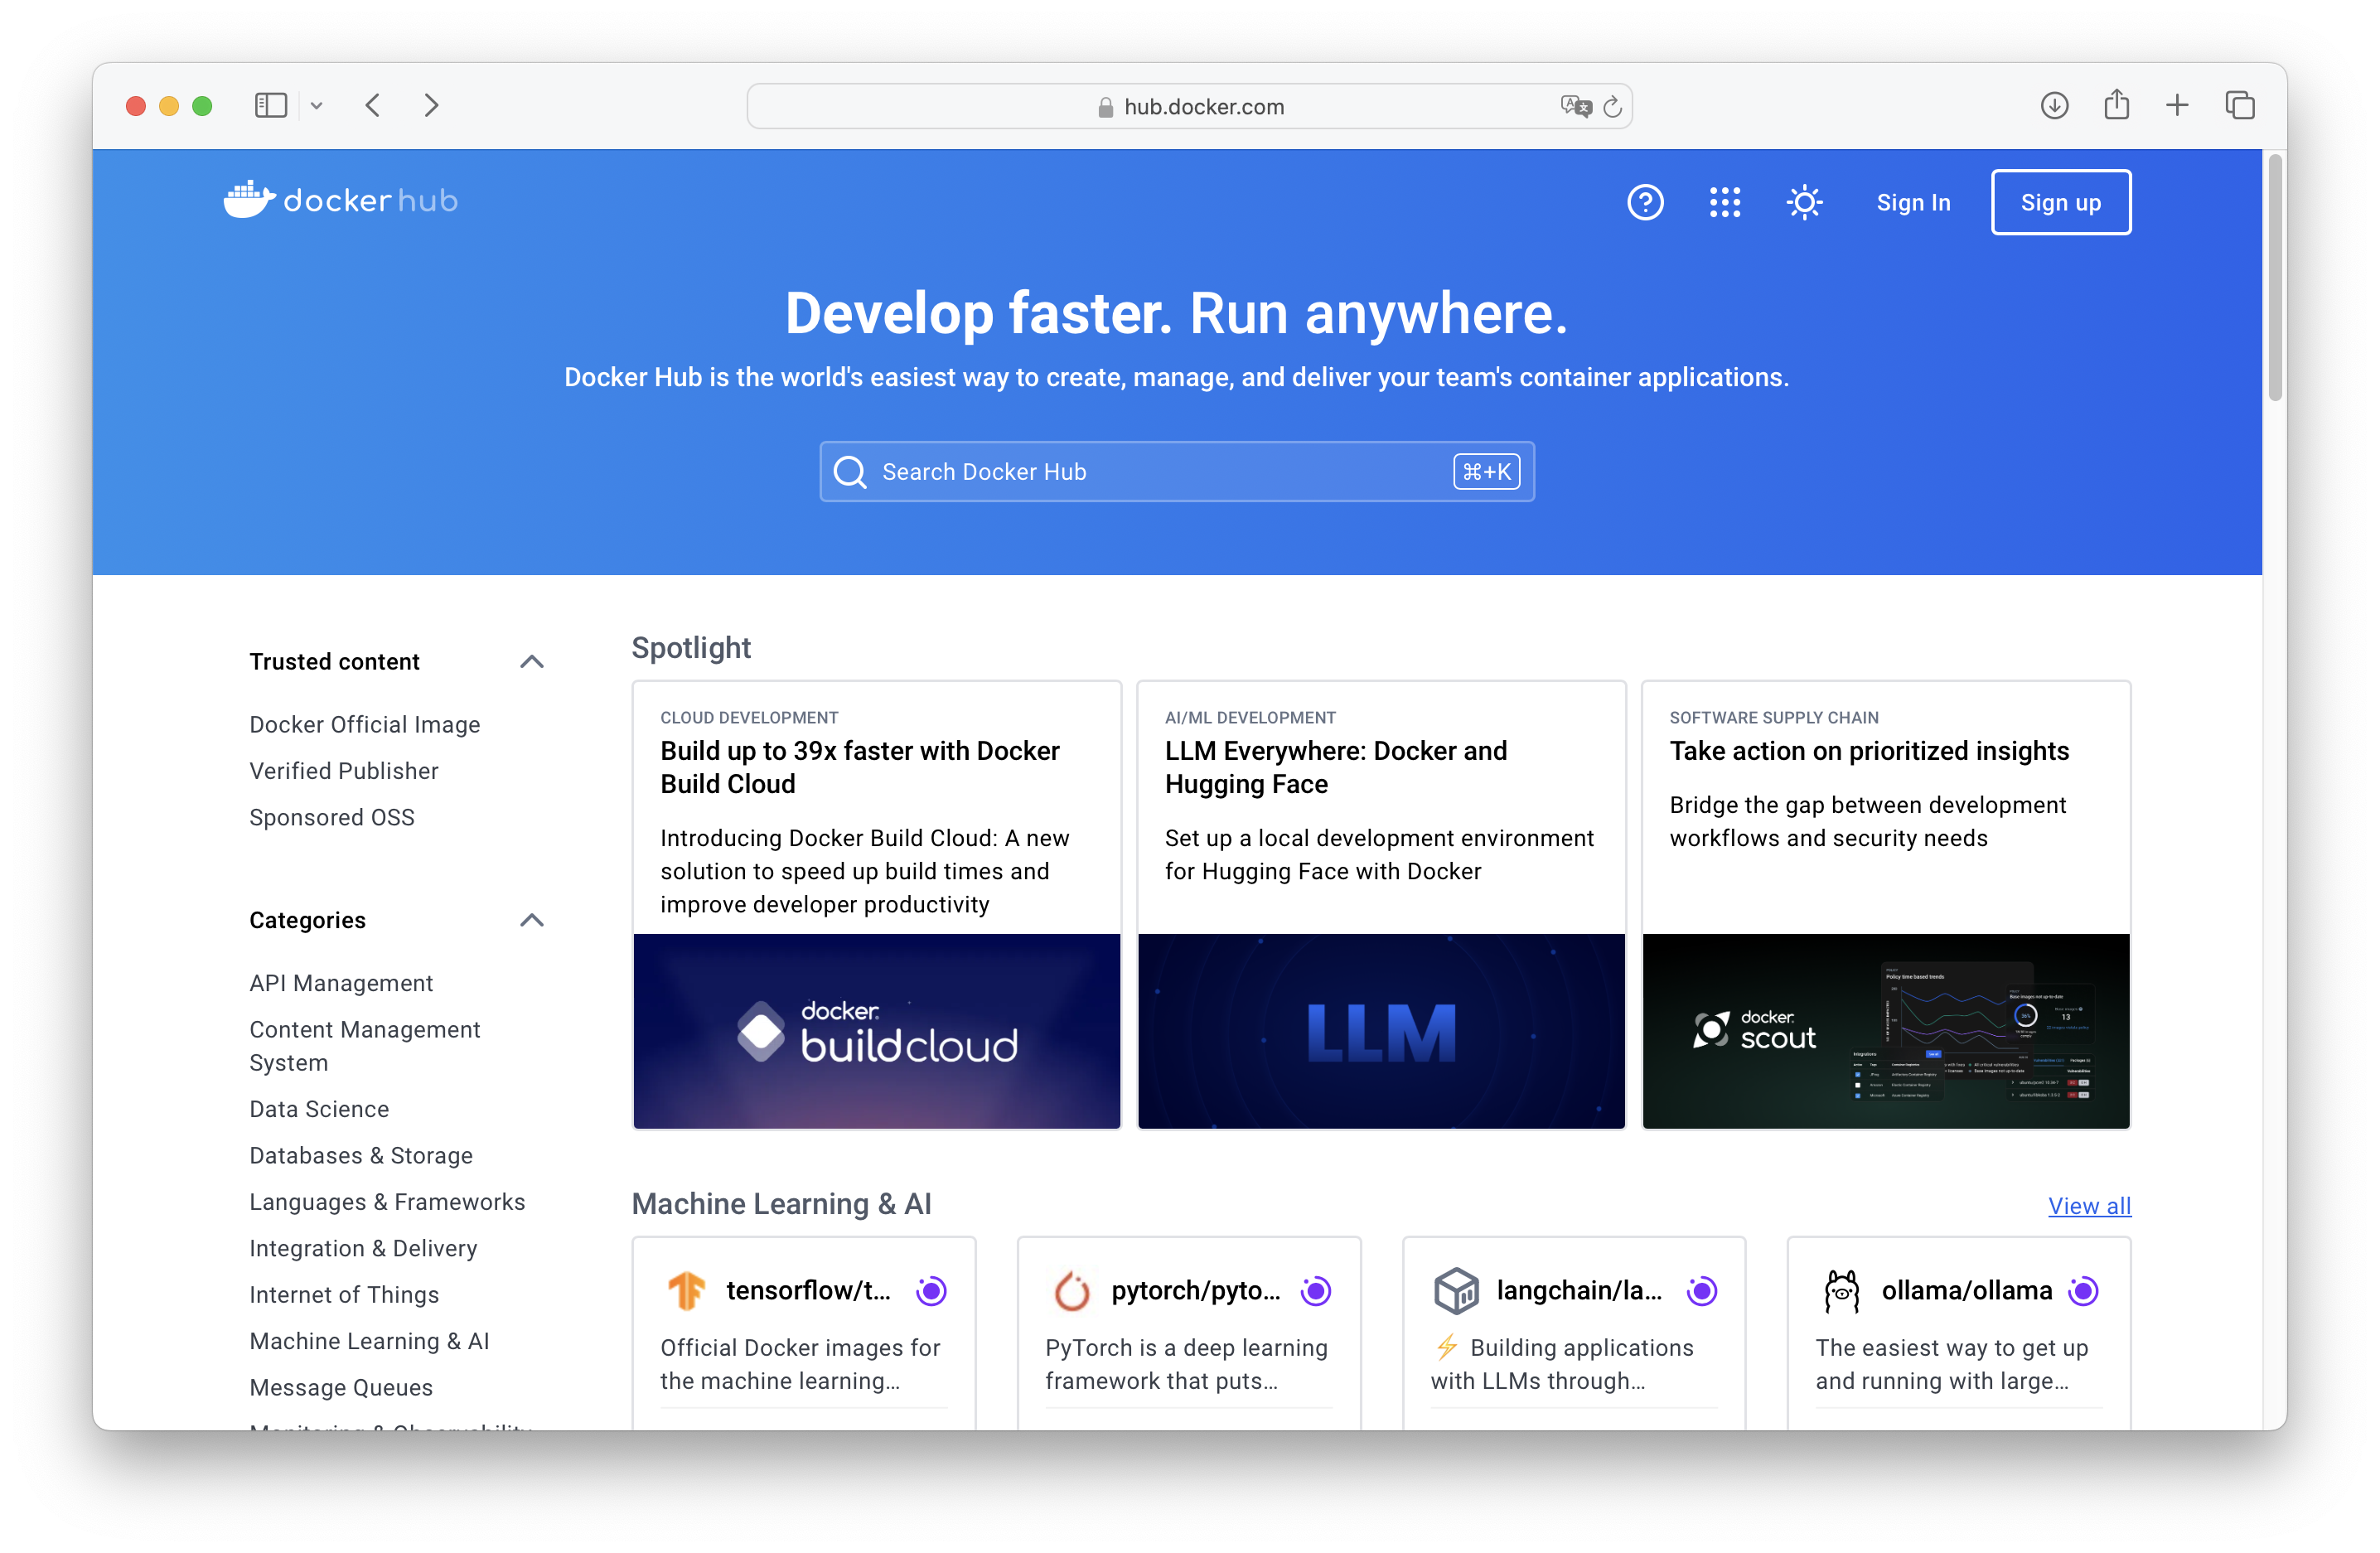
\includegraphics[width=.45\textwidth]{images/chapter4Images/ch4-2.png}
    \label{fig:zrGroup}
  }
  \caption{Docker Hub에서 static-site 이미지 가져오기}
  \label{fig:mainfig}
\end{figure*}

이 이미지는 Nginx 웹 서버를 실행하며, 이 서버는 컨테이너가 시작될 때 자동으로 시작됩니다. 이 이미지는 prakhar1989/static-site라는 이름으로 Docker Hub에 호스팅되었습니다. 이 이미지를 가져오고 실행하려면 다음 명령을 실행하세요.
\begin{lstlisting}[language=bash]
  $ sudo docker pull prakhar1989/static-site
  Using default tag: latest
  latest: Pulling from prakhar1989/static-site
  d4bce7fd68df: Pull complete 
  a3ed95caeb02: Pull complete 
  573113c4751a: Pull complete 
  31917632be33: Pull complete 
  77e66f18af1c: Pull complete 
  df3f108f3ade: Pull complete 
  d7a279eb19f5: Pull complete 
  e798589c05c5: Pull complete 
  78eeaf458ae0: Pull complete 
  Digest: sha256:bb6907c8db9ac4c6cadb25162a979e286575cd8b27727c08c7fbaf30988534db
  Status: Downloaded newer image for prakhar1989/static-site:latest
  docker.io/prakhar1989/static-site:latest
\end{lstlisting}

이미지가 로컬에 없으면 클라이언트가 먼저 레지스트리에서 이미지를 가져온 다음 이미지를 실행합니다. 모든 것이 잘 되면 터미널에 Nginx is running... 메시지가 표시됩니다. 이제 서버가 실행 중인데, 웹사이트를 어떻게 볼까요? 어떤 포트에서 실행되고 있나요? 더 중요한 것은 호스트 머신에서 컨테이너에 어떻게 액세스할까요? Ctrl+C를 눌러 컨테이너를 중지합니다.

이 경우 클라이언트가 포트를 노출하지 않으므로 포트를 게시하도록 docker run 명령을 다시 실행해야 합니다. 동시에 터미널이 실행 중인 컨테이너에 연결되지 않도록 해야 합니다. 이렇게 하면 터미널을 닫아도 컨테이너는 계속 실행됩니다. 이를 분리 모드라고 합니다.
\begin{lstlisting}[language=bash]
$ docker run -d -P --name static-site prakhar1989/static-site
e61d12292d69556eabe2a44c16cbd54486b2527e2ce4f95438e504afb7b02810
\end{lstlisting}

위 명령에서 -d는 터미널을 분리하고, -P는 모든 노출된 포트를 임의의 포트로 게시하며, --name은 컨테이너에 부여할 이름을 지정합니다. 이제 docker port [CONTAINER] 명령을 실행하여 포트를 확인할 수 있습니다.
\begin{lstlisting}[language=bash]
$ docker port static-site
80/tcp -> 0.0.0.0:32769
443/tcp -> 0.0.0.0:32768
\end{lstlisting}

브라우저에서 \url{http://localhost:32769}를 열 수 있습니다.
\begin{quote}
참고: docker-toolbox를 사용하는 경우 docker-machine ip default를 사용하여 IP를 가져와야 할 수 있습니다.
\end{quote}
클라이언트가 컨테이너로 연결을 전달할 포트를 지정할 수도 있습니다.
\begin{lstlisting}[language=bash]
$ docker run -p 8888:80 prakhar1989/static-site
Nginx is running...
\end{lstlisting}

\begin{figure}
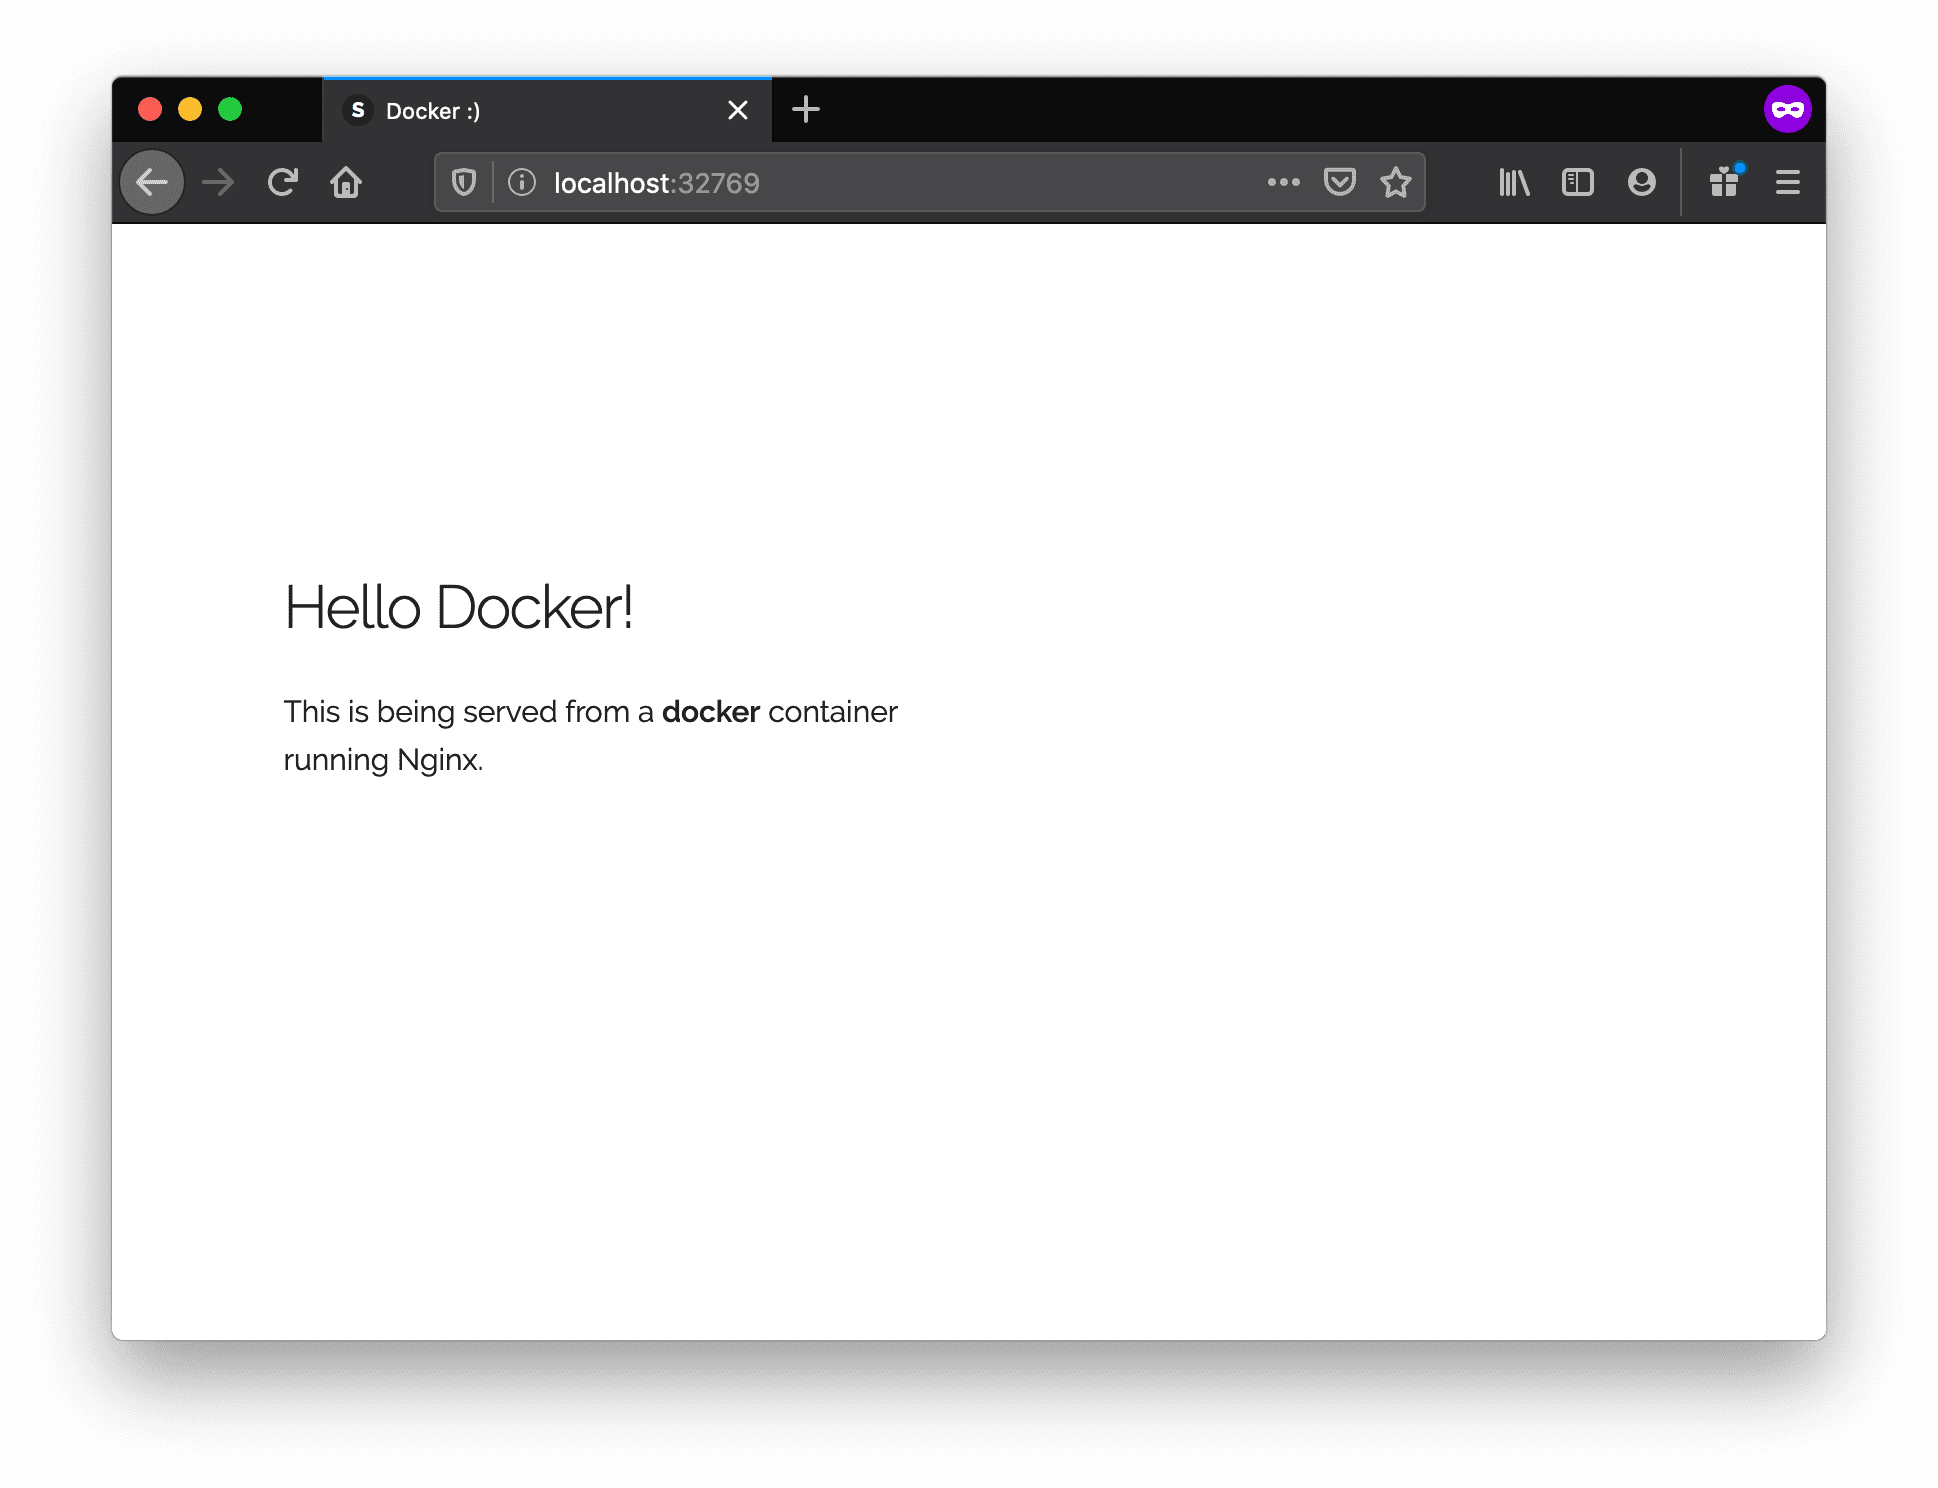
\includegraphics[width=\textwidth]{images/static.png}
\caption{Static Site}
\label{fig:static}
\end{figure}


분리된 컨테이너를 중지하려면 컨테이너 ID를 사용하여 docker stop 명령을 실행하세요. 이 경우 static-site라는 이름을 사용하여 컨테이너를 시작했습니다.
\begin{lstlisting}[language=bash]
$ docker stop static-site
static-site
\end{lstlisting}

매우 간단하죠. 실제 서버에 배포하려면 Docker를 설치하고 위 Docker 명령을 실행하면 됩니다. 이제 Docker 이미지를 사용하여 웹 서버를 실행하는 방법을 보았으므로, 자신만의 Docker 이미지를 생성하는 방법이 궁금할 것입니다. 다음 섹션에서 이를 탐구할 것입니다.

\section{Docker 이미지}
이미지를 이미 살펴보았지만, 이 섹션에서는 Docker 이미지가 무엇인지 더 자세히 살펴보고 직접 이미지를 만들어 보겠습니다! 마지막으로, 이 이미지를 사용하여 로컬에서 응용 프로그램을 실행하고 최종적으로 AWS에 배포하여 친구들과 공유할 것입니다! 흥미롭지 않나요? 그럼 시작해 봅시다.

Docker 이미지는 컨테이너의 기본입니다. 이전 예제에서는 Busybox 이미지를 레지스트리에서 가져와 Docker 클라이언트에 해당 이미지 기반의 컨테이너를 실행하도록 요청했습니다. 로컬에서 사용할 수 있는 이미지 목록을 보려면 docker images 명령을 사용하세요.
\begin{lstlisting}[language=bash]
$ docker images
REPOSITORY                      TAG                 IMAGE ID            CREATED             VIRTUAL SIZE
prakhar1989/catnip              latest              c7ffb5626a50        2 hours ago         697.9 MB
prakhar1989/static-site         latest              b270625a1631        21 hours ago        133.9 MB
python                          3-onbuild           cf4002b2c383        5 days ago          688.8 MB
martin/docker-cleanup-volumes   latest              b42990daaca2        7 weeks ago         22.14 MB
ubuntu                          latest              e9ae3c220b23        7 weeks ago         187.9 MB
busybox                         latest              c51f86c28340        9 weeks ago         1.109 MB
hello-world                     latest              0a6ba66e537a        11 weeks ago        960 B
\end{lstlisting}

위에는 레지스트리에서 가져온 이미지 목록과 직접 생성한 이미지 목록이 표시됩니다(곧 볼 수 있습니다). TAG는 이미지의 특정 스냅샷을 나타내며 IMAGE ID는 해당 이미지의 고유 식별자입니다.

간단히 말해, 이미지를 git 저장소와 유사하게 생각할 수 있습니다 - 이미지는 변경 사항을 커밋할 수 있으며 여러 버전을 가질 수 있습니다. 특정 버전 번호를 제공하지 않으면 클라이언트는 기본적으로 latest로 설정됩니다. 예를 들어, ubuntu 이미지의 특정 버전을 가져올 수 있습니다.
\begin{lstlisting}[language=bash]
$ docker pull ubuntu:18.04
\end{lstlisting}

새 Docker 이미지를 얻으려면 레지스트리(Docker Hub와 같은)에서 가져오거나 직접 생성할 수 있습니다. Docker Hub에는 수만 개의 이미지가 있습니다. 커맨드 라인을 사용하여 docker search로 이미지를 검색할 수도 있습니다.

이미지와 관련하여 주의해야 할 중요한 차이점은 기본 이미지와 자식 이미지의 차이입니다.
\begin{itemize}
    \item \textbf{기본 이미지}는 부모 이미지가 없는 이미지로, 보통 ubuntu, busybox 또는 debian과 같은 운영 체제가 있는 이미지입니다.
    \item \textbf{자식 이미지}는 기본 이미지를 기반으로 추가 기능을 제공하는 이미지입니다.
\end{itemize}

그다음으로 공식 이미지와 사용자 이미지가 있으며, 이 둘 다 기본 이미지와 자식 이미지가 될 수 있습니다.
\begin{itemize}
    \item \textbf{공식 이미지}는 Docker 팀에서 공식적으로 유지 관리하고 지원하는 이미지입니다. 이러한 이미지는 일반적으로 한 단어로 이루어져 있습니다. 위의 이미지 목록에서 python, ubuntu, busybox 및 hello-world 이미지는 공식 이미지입니다.
    \item \textbf{사용자 이미지}는 사용자(여러분과 같은)가 생성하고 공유한 이미지입니다. 기본 이미지를 기반으로 추가 기능을 제공합니다. 일반적으로 user/image-name 형식으로 작성됩니다.
\end{itemize}

\section{우리의 첫 번째 이미지}
이미지에 대한 이해가 깊어졌으니 이제 직접 이미지를 만들어 봅시다. 이 섹션의 목표는 간단한 Flask 응용 프로그램을 샌드박싱하는 이미지를 만드는 것입니다. 이 튜토리얼을 위해 귀여운 작은 Flask 앱을 이미 만들어 두었으며, 이 앱은 로드될 때마다 랜덤한 고양이 gif를 표시합니다. 고양이를 좋아하지 않는 사람이 누가 있겠습니까? 아직 하지 않았다면 다음 명령을 사용하여 로컬 저장소를 클론하세요 -
\begin{lstlisting}[language=bash]
$ git clone https://github.com/prakhar1989/docker-curriculum.git
$ cd docker-curriculum/flask-app
\end{lstlisting}

\begin{quote}
이 작업은 docker 명령을 실행하는 머신에서 클론해야 하며, Docker 컨테이너 내부에서는 클론하지 마세요.
\end{quote}

다음 단계는 이 웹 앱을 포함하는 이미지를 만드는 것입니다. 위에서 언급한 것처럼 모든 사용자 이미지는 기본 이미지를 기반으로 합니다. 우리의 응용 프로그램이 Python으로 작성되었기 때문에 사용할 기본 이미지는 Python 3가 될 것입니다.

\section{Dockerfile}
Dockerfile은 이미지 생성 시 Docker 클라이언트가 호출하는 명령 목록이 포함된 간단한 텍스트 파일입니다. 이미지 생성 프로세스를 자동화하는 간단한 방법입니다. 가장 좋은 점은 Dockerfile에서 작성하는 명령이 리눅스 명령과 거의 동일하다는 것입니다. 따라서 Dockerfile을 작성하기 위해 새로운 문법을 배울 필요가 없습니다.

응용 프로그램 디렉토리에 Dockerfile이 포함되어 있지만 처음으로 이 작업을 수행하므로 처음부터 새로 만들겠습니다. 좋아하는 텍스트 편집기에서 빈 파일을 생성하고 flask 앱과 같은 폴더에 Dockerfile이라는 이름으로 저장하세요.

기본 이미지를 지정하는 것부터 시작합니다. FROM 키워드를 사용하세요 -
\begin{lstlisting}[language=dockerfile]
FROM python:3.8
\end{lstlisting}

다음 단계는 파일을 복사하고 종속성을 설치하는 명령을 작성하는 것입니다. 먼저 작업 디렉토리를 설정한 다음 응용 프로그램의 모든 파일을 복사합니다.
\begin{lstlisting}[language=dockerfile]
# Set the working directory for the application
WORKDIR /usr/src/app
# Copy all files to the container
COPY . .
\end{lstlisting}

이제 파일을 복사했으므로 종속성을 설치할 수 있습니다.
\begin{lstlisting}[language=dockerfile]
# Install dependencies
RUN pip install --no-cache-dir -r requirements.txt
\end{lstlisting}

다음으로 노출해야 할 포트 번호를 지정해야 합니다. Flask 앱이 5000 포트에서 실행되므로 이를 표시하겠습니다.
\begin{lstlisting}[language=dockerfile]
EXPOSE 5000
\end{lstlisting}

마지막 단계는 응용 프로그램을 실행하는 명령을 작성하는 것입니다. 이는 단순히 python ./app.py입니다. 이를 위해 CMD 명령을 사용합니다 -
\begin{lstlisting}[language=dockerfile]
CMD [ "python", "./app.py" ]
\end{lstlisting}

CMD의 주요 목적은 컨테이너 시작 시 실행할 명령을 지정하는 것입니다. 이렇게 하면 Dockerfile이 준비됩니다. 다음과 같이 보일 것입니다 -
\begin{lstlisting}[language=dockerfile]
FROM python:3.8

# Set the working directory for the application
WORKDIR /usr/src/app
# Copy all files to the container
COPY . .
# Install dependencies
RUN pip install --no-cache-dir -r requirements.txt
# Define the port number the container should expose
EXPOSE 5000
# Run the command
CMD ["python", "./app.py"]
\end{lstlisting}

이제 Dockerfile이 준비되었으므로 이미지를 빌드할 수 있습니다. docker build 명령은 Dockerfile에서 Docker 이미지를 생성하는 작업을 수행합니다.

아래 섹션에서는 동일한 명령을 실행한 출력을 보여줍니다. 명령을 직접 실행하기 전에(점을 잊지 마세요) 제 사용자 이름을 여러분의 사용자 이름으로 바꾸세요. 이 사용자 이름은 Docker Hub에 등록할 때 생성한 사용자 이름과 동일해야 합니다. 아직 계정을 생성하지 않았다면, 지금 바로 생성해 주세요. docker build 명령은 매우 간단합니다 - 선택적으로 -t와 위치를 사용하여 태그 이름과 Dockerfile이 포함된 디렉토리를 지정할 수 있습니다.
\begin{lstlisting}[language=bash]
$ docker build -t yourusername/catnip .
Sending build context to Docker daemon 8.704 kB
Step 1 : FROM python:3.8
# Executing 3 build triggers...
Step 1 : COPY requirements.txt /usr/src/app/
 ---> Using cache
Step 1 : RUN pip install --no-cache-dir -r requirements.txt
 ---> Using cache
Step 1 : COPY . /usr/src/app
 ---> 1d61f639ef9e
Removing intermediate container 4de6ddf5528c
Step 2 : EXPOSE 5000
 ---> Running in 12cfcf6d67ee
 ---> f423c2f179d1
Removing intermediate container 12cfcf6d67ee
Step 3 : CMD python ./app.py
 ---> Running in f01401a5ace9
 ---> 13e87ed1fbc2
Removing intermediate container f01401a5ace9
Successfully built 13e87ed1fbc2
\end{lstlisting}

python:3.8 이미지를 가지고 있지 않다면, 클라이언트가 먼저 이미지를 가져오고 나서 여러분의 이미지를 생성할 것입니다. 따라서 명령을 실행한 출력은 저와 다를 것입니다. 모든 것이 잘 되었다면, 이미지는 준비되었을 것입니다! docker images를 실행하여 이미지가 표시되는지 확인하세요.

이 섹션의 마지막 단계는 이미지를 실행하고 실제로 작동하는지 확인하는 것입니다(제 사용자 이름을 여러분의 사용자 이름으로 바꾸세요).
\begin{lstlisting}[language=bash]
$ docker run -p 8888:5000 yourusername/catnip
 * Running on http://0.0.0.0:5000/ (Press CTRL+C to quit)
\end{lstlisting}

방금 실행한 명령은 컨테이너 내부의 서버에 5000 포트를 사용하고 이를 외부적으로 8888 포트에서 노출했습니다. 8888 포트를 사용하는 URL로 이동하면 앱이 활성화된 것을 볼 수 있습니다.

\begin{figure}
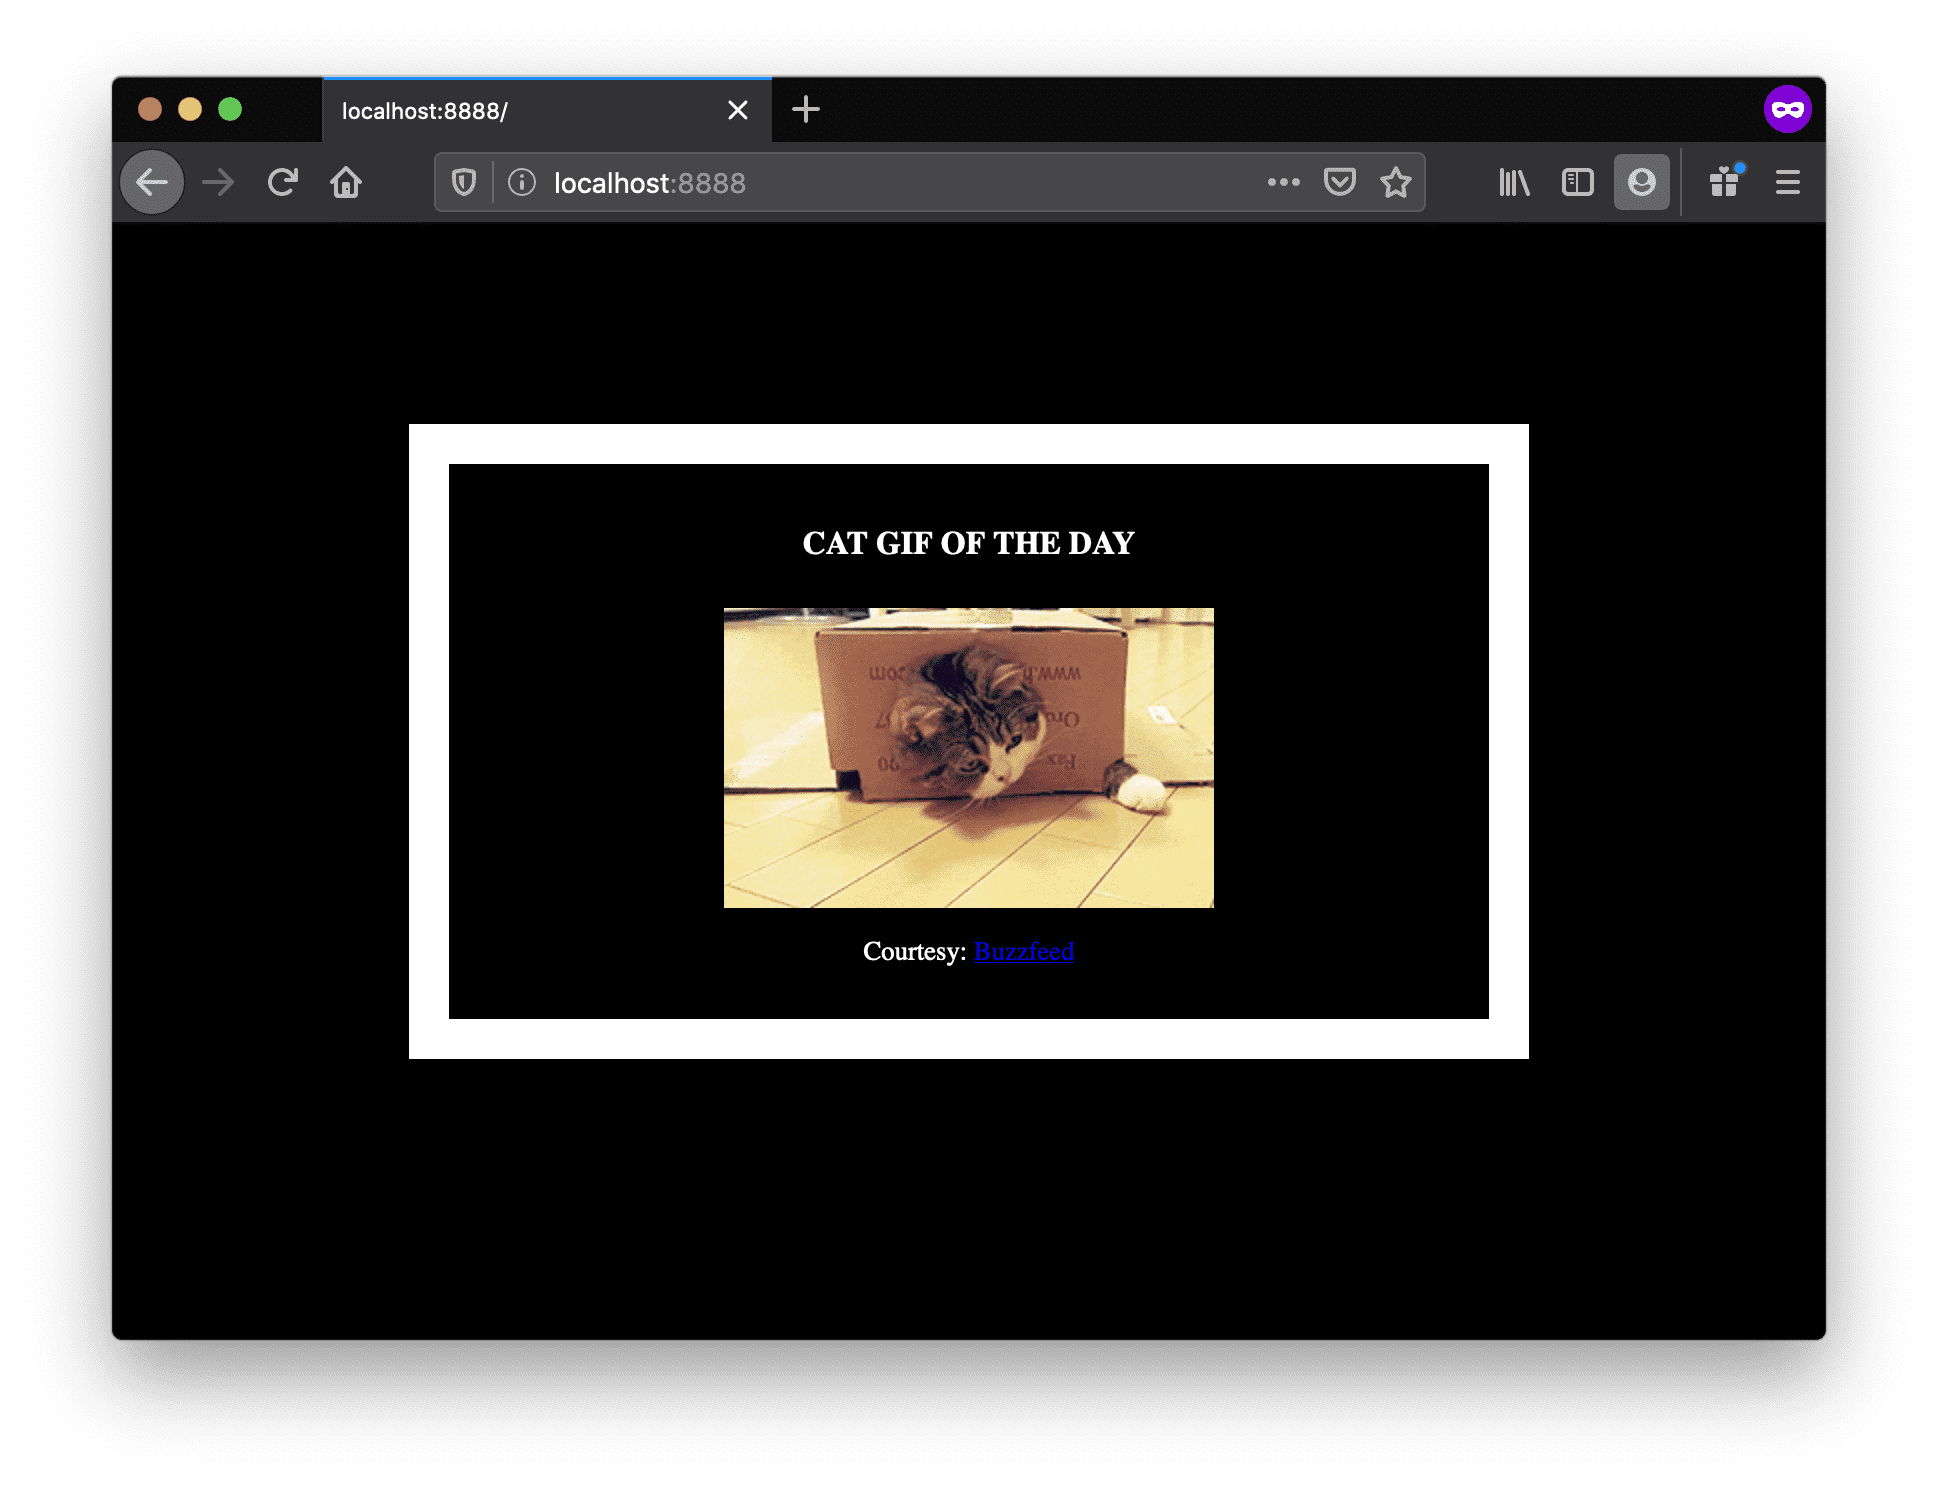
\includegraphics[width=\textwidth]{images/catgif.png}
\caption{Cat GIF Website}
\end{figure}

축하합니다! 첫 번째 Docker 이미지를 성공적으로 생성했습니다.

\section{AWS에서 Docker}
응용 프로그램을 친구와 공유할 수 없다면 무슨 소용이 있을까요? 이 섹션에서는 응용 프로그램을 클라우드에 배포하여 친구와 공유할 수 있도록 하는 방법을 살펴보겠습니다! 우리는 AWS Elastic Beanstalk을 사용하여 몇 번의 클릭만으로 응용 프로그램을 실행할 것입니다. 또한 Beanstalk을 사용하여 응용 프로그램을 확장하고 관리하는 것이 얼마나 쉬운지 볼 것입니다!

\subsection{Docker push}
AWS에 앱을 배포하기 전에 해야 할 첫 번째 일은 AWS에서 접근할 수 있는 레지스트리에 이미지를 게시하는 것입니다. 사용할 수 있는 Docker 레지스트리에는 여러 가지가 있습니다(자신만의 레지스트리를 호스팅할 수도 있습니다). 지금은 Docker Hub를 사용하여 이미지를 게시하겠습니다.

이미지를 처음으로 푸시하는 경우 클라이언트가 로그인하라는 메시지를 표시할 것입니다. Docker Hub에 로그인할 때 사용한 것과 동일한 자격 증명을 제공하세요.
\begin{lstlisting}[language=bash]
$ docker login
Login in with your Docker ID to push and pull images from Docker Hub. If you do not have a Docker ID, head over to https://hub.docker.com to create one.
Username: yourusername
Password:
WARNING! Your password will be stored unencrypted in /Users/yourusername/.docker/config.json
Configure a credential helper to remove this warning. See https://docs.docker.com/engine/reference/commandline/login/credential-store

Login Succeeded
\end{lstlisting}

게시하려면 위 이미지 태그의 이름을 여러분의 이름으로 바꾸는 것을 기억하면서 아래 명령을 입력하세요. 클라이언트가 어디에 게시할지 알 수 있도록 $yourusername/image_name$ 형식을 유지하는 것이 중요합니다.
\begin{lstlisting}[language=bash]
$ docker push yourusername/catnip
\end{lstlisting}

이 작업이 완료되면 Docker Hub에서 여러분의 이미지를 볼 수 있습니다. 예를 들어, 여기는 제 이미지의 웹 페이지입니다.
\begin{quote}
참고: 앞으로 나아가기 전에 명확히 하고 싶은 것은, AWS에 배포하기 위해 이미지를 공개 레지스트리(또는 어떤 레지스트리)에 호스팅하는 것이 필수적이지 않다는 것입니다. 다음 백만 달러 스타트업을 위한 코드를 작성하는 경우 이 단계를 건너뛸 수 있습니다. 이미지를 공개적으로 푸시하는 이유는 중간 구성 단계를 건너뛰어 배포를 매우 간단하게 만들기 때문입니다.
\end{quote}
이제 여러분의 이미지가 온라인에 있으므로 Docker가 설치된 누구나 단일 명령으로 여러분의 앱을 사용할 수 있습니다.
\begin{lstlisting}[language=bash]
$ docker run -p 8888:5000 yourusername/catnip
\end{lstlisting}

로컬 개발 환경 설정 / 응용 프로그램 구성을 공유하는 데 어려움을 겪은 적이 있다면, 이것이 얼마나 멋진 것인지 알 것입니다. 이것이 Docker가 멋진 이유입니다!

\subsection{Beanstalk}
AWS Elastic Beanstalk (EB)은 AWS에서 제공하는 PaaS (Platform as a Service)입니다. Heroku, Google App Engine 등을 사용해 본 적이 있다면 익숙할 것입니다. 개발자로서 여러분은 EB에게 앱을 어떻게 실행할지 알려주기만 하면 나머지는 EB가 처리합니다 - 확장, 모니터링 및 업데이트를 포함하여. 2014년 4월에 EB는 단일 컨테이너 Docker 배포를 지원하기 시작했으며, 이를 사용하여 앱을 배포할 것입니다. EB는 매우 직관적인 CLI를 가지고 있지만, 일부 설정이 필요하므로 간단하게 유지하기 위해 웹 UI를 사용하여 응용 프로그램을 시작하겠습니다.

따라하려면 기능하는 AWS 계정이 필요합니다. 아직 계정이 없으신 분은 지금 바로 만들어 주세요 - 신용 카드 정보를 입력해야 합니다. 걱정하지 마세요, 무료입니다. 이 튜토리얼에서 하는 모든 작업도 무료입니다! 시작해 봅시다.

단계는 다음과 같습니다:
\begin{itemize}
    \item AWS 콘솔에 로그인하세요.
    \item Elastic Beanstalk을 클릭하세요. 왼쪽 상단의 컴퓨팅 섹션에 있을 것입니다. 또는 Elastic Beanstalk 콘솔에 액세스할 수 있습니다.
\end{itemize}

\begin{figure}
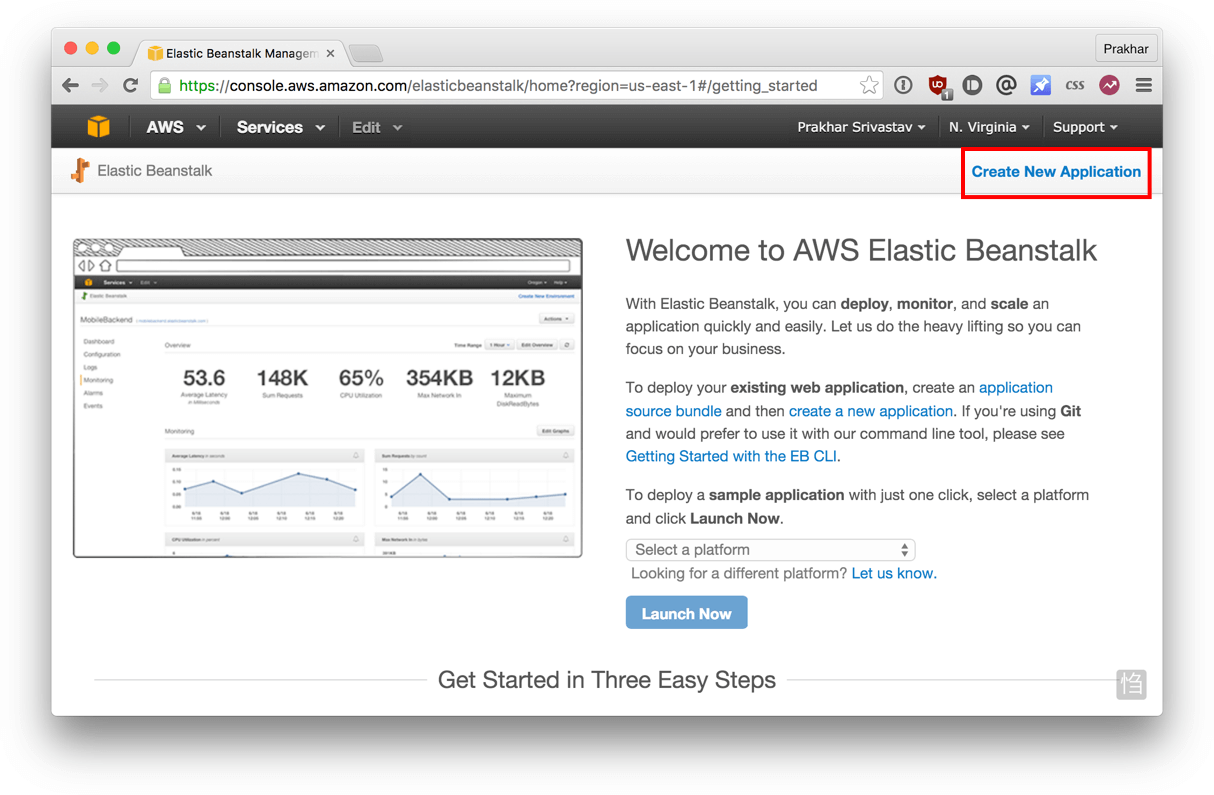
\includegraphics[width=\textwidth]{images/eb-start.png}
\caption{Elastic Beanstalk Start}
\label{fig:eb-start}
\end{figure}


\begin{itemize}
    \item 오른쪽 상단의 "새 응용 프로그램 생성"을 클릭하세요.
    \item 기억할 수 있는(그러나 고유한) 이름을 입력하고(선택 사항) 설명을 입력하세요.
    \item 새 환경 화면에서 새 환경을 만들고 웹 서버 환경을 선택하세요.
    \item 도메인을 선택하여 환경 정보를 입력하세요. 이 URL은 친구와 공유할 URL이므로 기억하기 쉬운 것으로 선택하세요.
    \item 기본 구성 섹션에서 미리 정의된 플랫폼에서 Docker를 선택하세요.
\end{itemize}

\begin{figure}
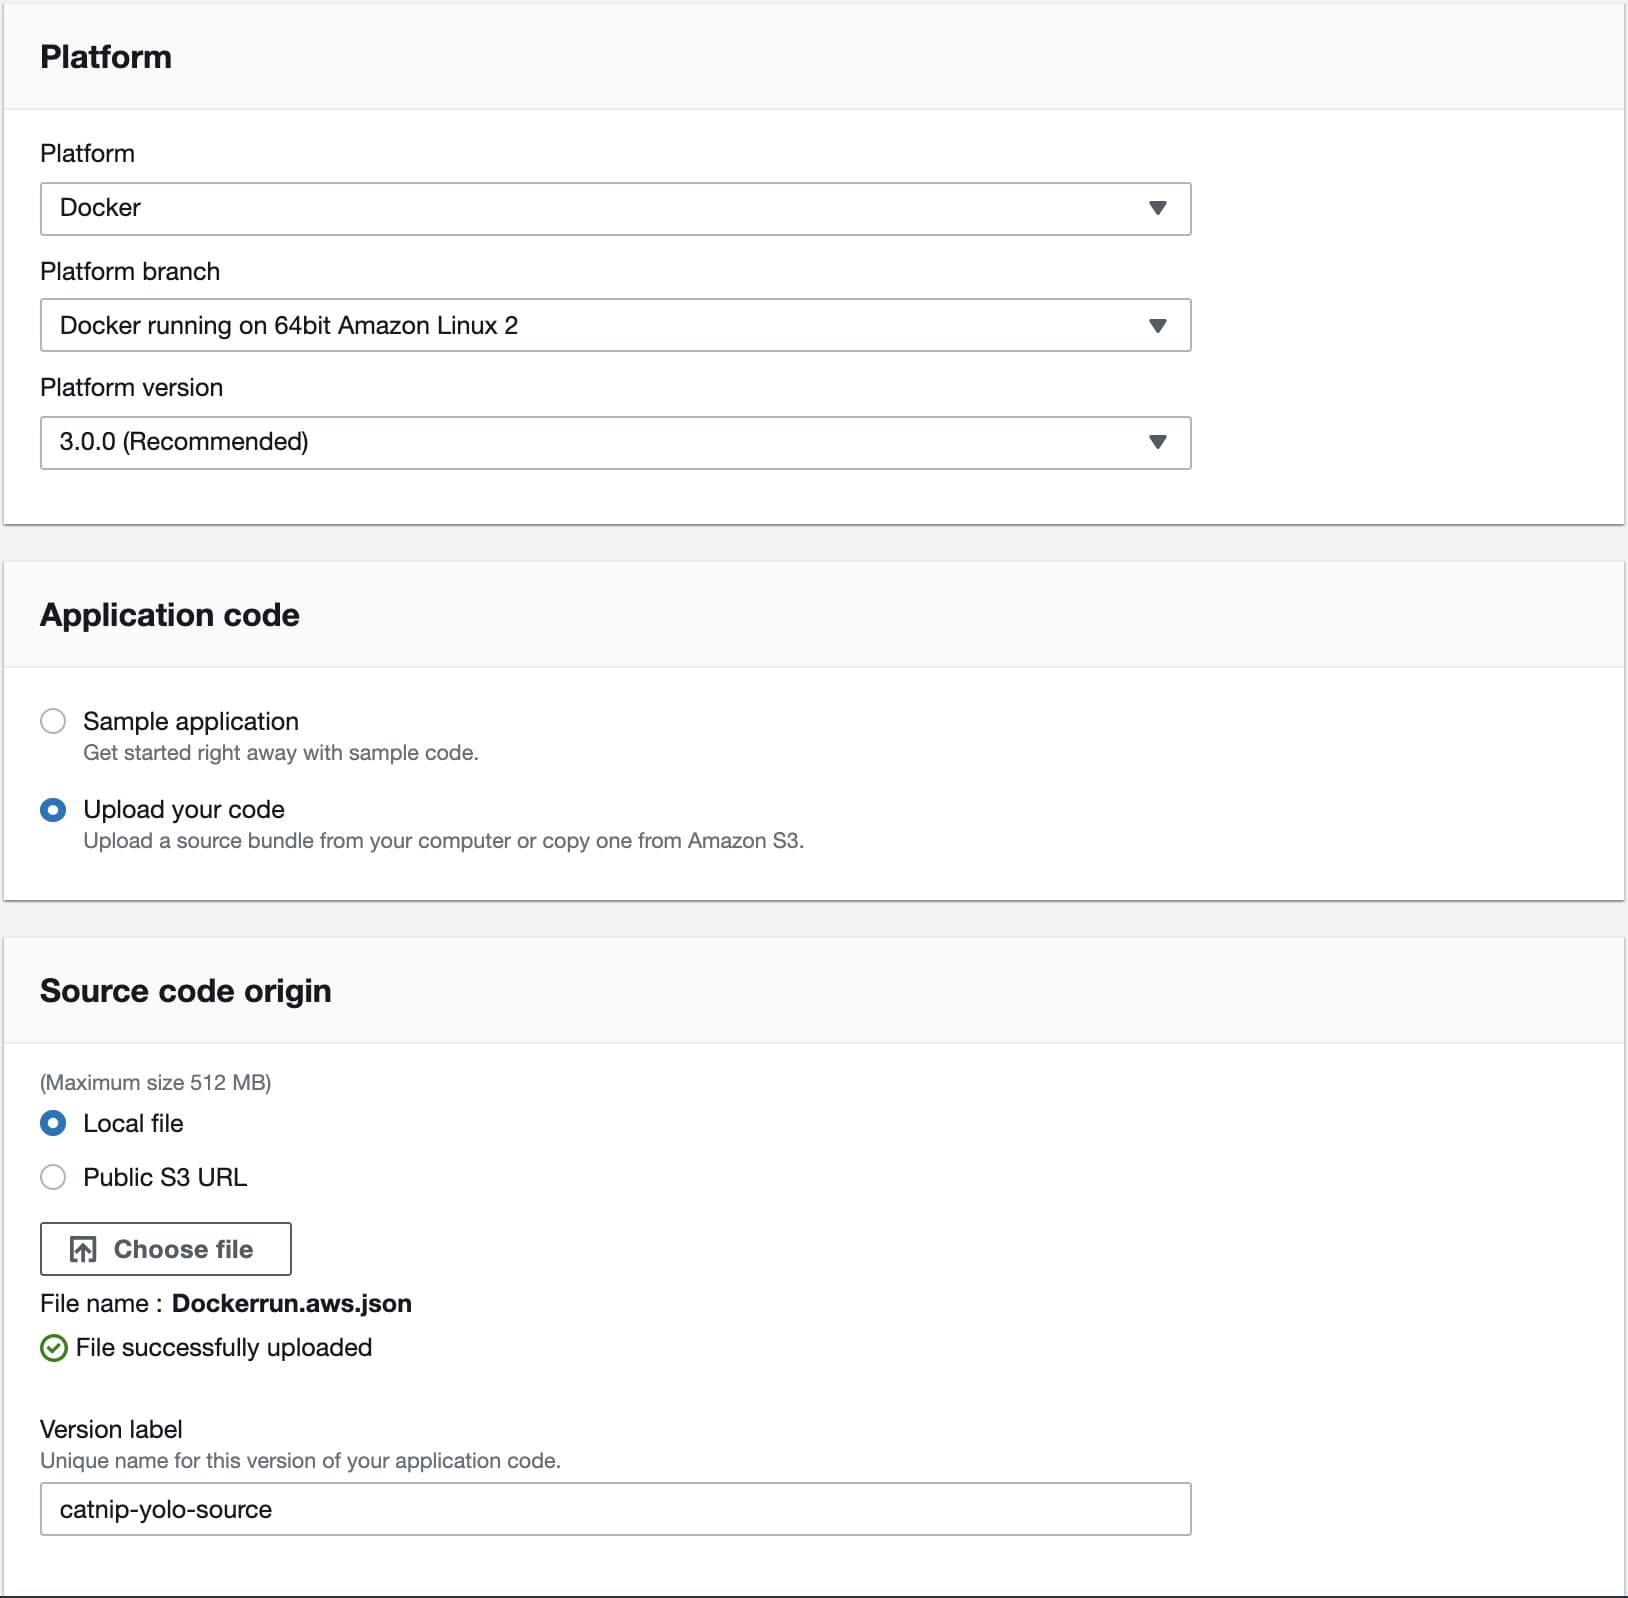
\includegraphics[width=\textwidth]{images/eb-docker.jpeg}
\caption{Elastic Beanstalk Environment Type}
\end{figure}


\begin{itemize}
    \item 이제 응용 프로그램 코드를 업로드해야 합니다. 그러나 응용 프로그램이 Docker 컨테이너로 패키징되었기 때문에 EB에게 컨테이너에 대해 알려주기만 하면 됩니다. flask-app 폴더에 있는 Dockerrun.aws.json 파일을 열고 이미지의 이름을 자신의 이미지 이름으로 편집하세요. 파일 내용을 곧 설명하겠습니다. 완료되면 "코드 업로드" 라디오 버튼을 선택하고 이 파일을 선택한 다음 "업로드"를 클릭하세요.
    \item "환경 생성"을 클릭하세요. 최종 화면에 환경이 설정 중이라는 스피너가 표시됩니다. 처음 설정에는 약 5분이 걸립니다.
\end{itemize}
기다리는 동안 Dockerrun.aws.json 파일에 무엇이 들어 있는지 간략히 살펴보겠습니다. 이 파일은 AWS 전용 파일로, EB에게 응용 프로그램 및 Docker 구성에 대한 세부 정보를 제공합니다.
\begin{lstlisting}[language=dockerfile]
{
  "AWSEBDockerrunVersion": "1",
  "Image": {
    "Name": "prakhar1989/catnip",
    "Update": "true"
  },
  "Ports": [
    {
      "ContainerPort": 5000,
      "HostPort": 8000
    }
  ],
  "Logging": "/var/log/nginx"
}
\end{lstlisting}

파일은 매우 간단하지만, 공식 문서를 참조하여 더 많은 정보를 얻을 수 있습니다. EB에게 사용할 이미지의 이름과 컨테이너가 열어야 할 포트를 제공합니다.

이제 인스턴스가 준비되었을 것입니다. EB 페이지로 이동하면 앱이 활성화되고 있는지 표시하는 녹색 체크 표시를 볼 수 있습니다.
\begin{figure}
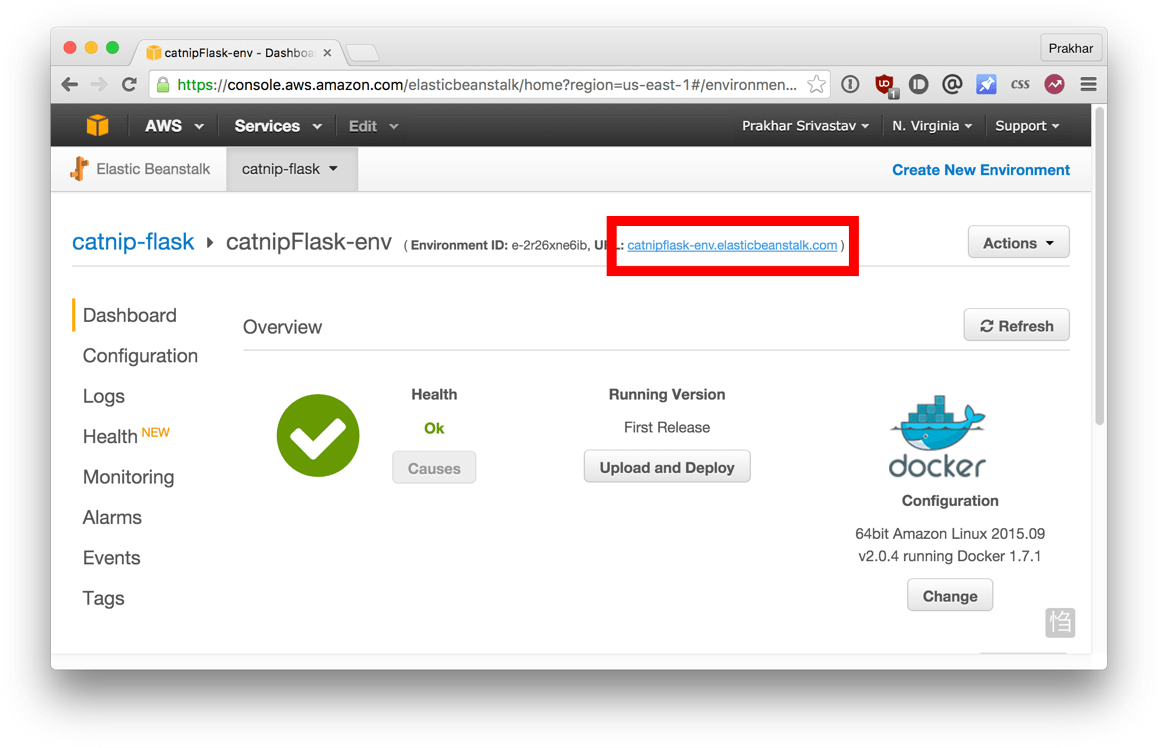
\includegraphics[width=\textwidth]{images/eb-deploy.png}
\caption{EB Deploy}
\end{figure}



브라우저에서 URL을 열고 응용 프로그램이 실행되는 것을 확인하세요. 이 링크를 친구와 가족에게 이메일 / IM / 스냅챗으로 보내서 고양이 gif를 즐길 수 있도록 하세요.

\subsection{정리}
응용 프로그램의 영광을 즐긴 후에는 추가 리소스에 대한 비용이 청구되지 않도록 환경을 종료하는 것을 잊지 마세요.

\begin{figure}
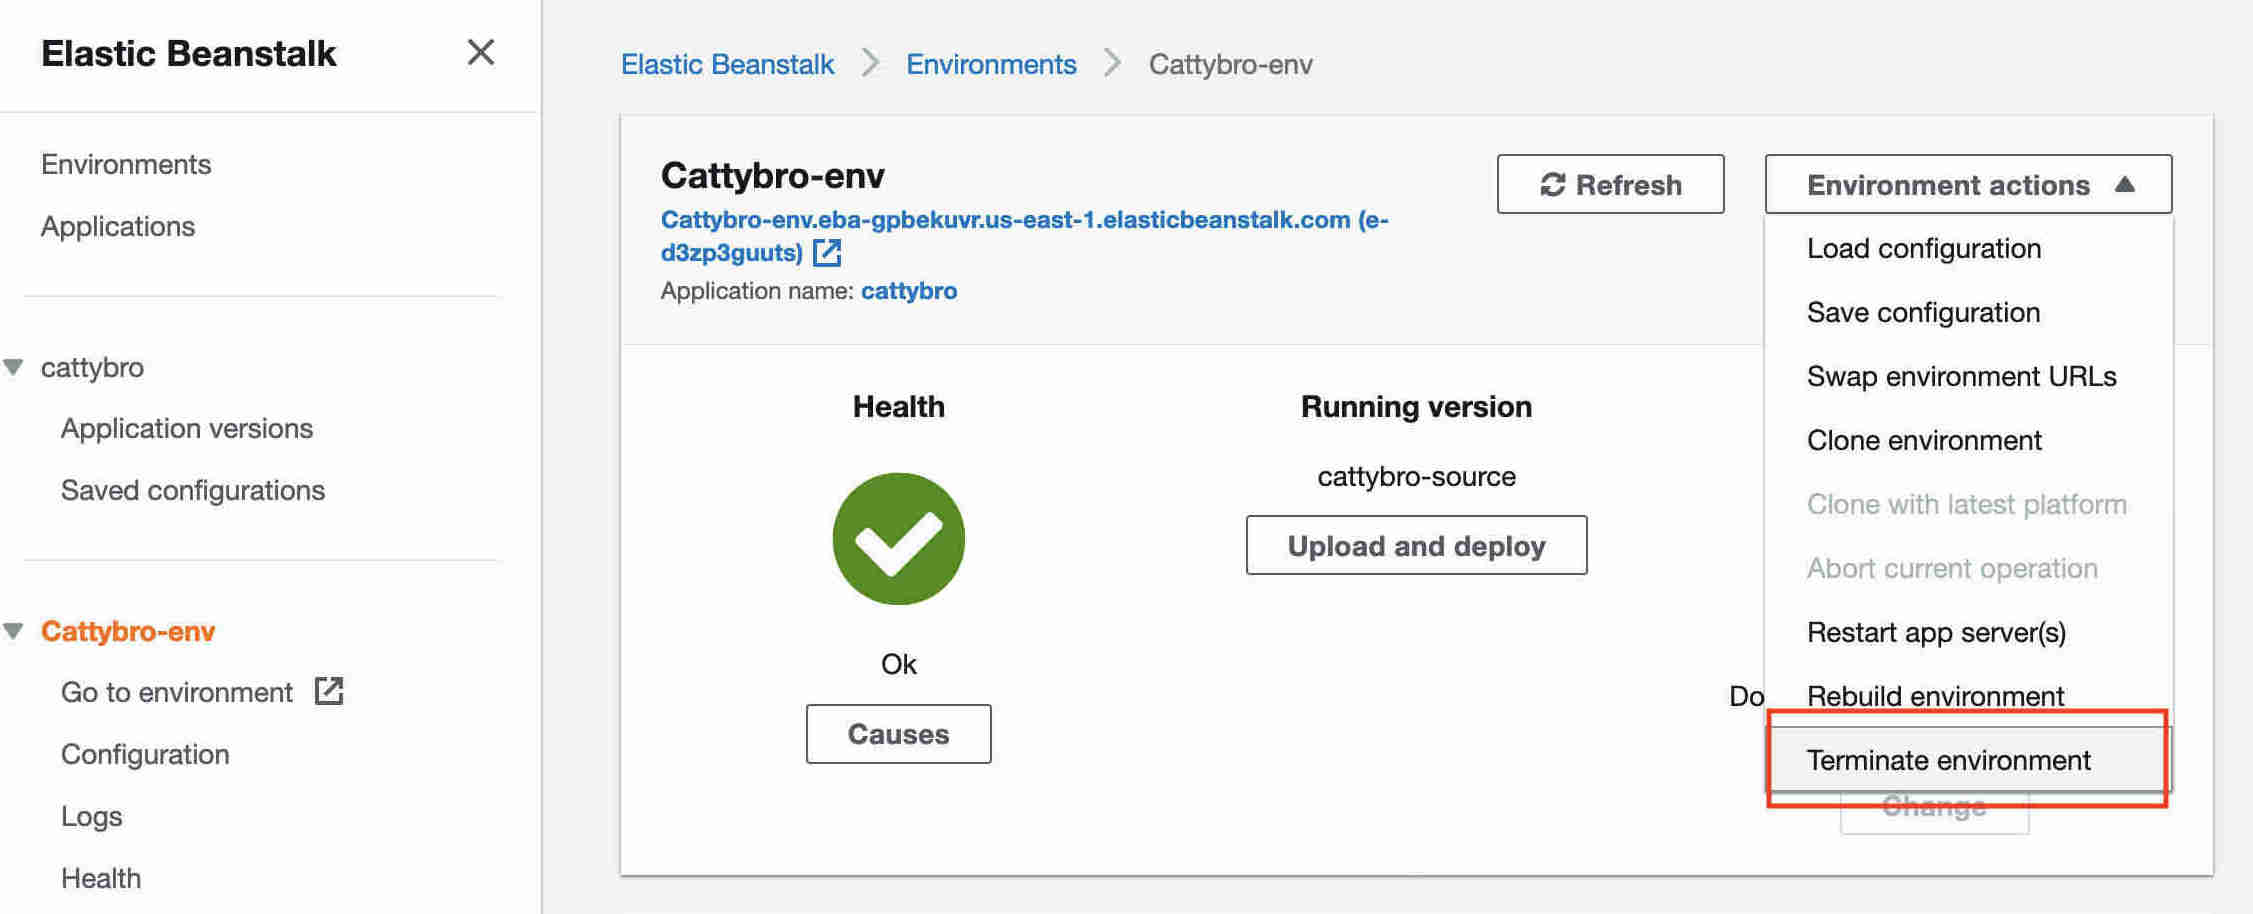
\includegraphics[width=\textwidth]{images/eb-terminate.jpg}
\caption{Terminate EB}
\end{figure}


축하합니다! 첫 번째 Docker 응용 프로그램을 배포했습니다! 많은 단계처럼 보일 수 있지만, EB의 커맨드 라인 도구를 사용하면 Heroku의 기능을 몇 번의 키 스트로크로 거의 모방할 수 있습니다! Docker가 클라우드에서 응용 프로그램을 구축하고 배포하는 많은 어려움을 덜어준다는 것에 동의하시길 바랍니다. AWS의 단일 컨테이너 Docker 환경에 대한 문서를 읽어보시길 권장합니다.

튜토리얼의 마지막 부분에서는 좀 더 복잡한 실제 환경을 모방하는 응용 프로그램을 배포할 것입니다. 영구적인 백엔드 저장소 계층이 있는 앱입니다. 바로 시작해 봅시다!